% SC1005 --- Chapter 4: Sequential Logic --- Latches & Flip-Flops (0->100)
\chapter{Sequential Logic: Latches and Flip-Flops}
\label{ch:sequential}

\begin{quote}
\emph{``Combinational circuits forget; sequential circuits remember.''}
Add feedback and you get memory. This chapter builds memory from first principles:
SR latch $\to$ D latch $\to$ master-slave $\to$ edge-triggered flip-flop.
\end{quote}

\noindent\fbox{\parbox{\dimexpr\linewidth-2\fboxsep-2\fboxrule}{%
\textbf{From zero: memory from wires.} We assume only gates (Ch.~\ref{ch:boolean}--\ref{ch:combinational}).
We add one idea---feedback---and derive every latch/flop from it. No prior sequential knowledge.}}
\vspace{0.4em}

\section*{Learning Outcomes}
After this chapter you will be able to:
\begin{enumerate}[label=(L\arabic*)]
    \item distinguish combinational from sequential and explain the role of feedback;
    \item analyse SR and D latches built from NAND/NOR gates;
    \item explain master-slave and edge-triggered D and JK flip-flops;
    \item describe setup/hold, propagation delay, and the clock concept;
    \item use characteristic tables and excitation tables for analysis.
\end{enumerate}

% ============================================================
\section{Why Feedback? From Combinational to Sequential}
\label{sec:feedback}
A combinational output depends only on \emph{present} inputs. Add a wire from output back to
input and output now depends on \emph{history}---that is memory. The simplest feedback loop is
two cross-coupled inverters (a bistable): two stable states $0$ and $1$, holding one bit forever
until forced to flip. All latches/flops elaborate this bistable core with control inputs.

A \emph{clock} (periodic square wave) disciplines when state may change, avoiding races.
\emph{Level-sensitive} (latch) follows the input while the clock is high; \emph{edge-triggered}
(flip-flop) samples only on a clock edge ($\uparrow$ rising, $\downarrow$ falling).

\section{SR Latch: The Simplest Memory}
\label{sec:sr-latch}
Cross-coupled NOR (or NAND) gates give Set-Reset behaviour: $S=1$ sets $Q=1$, $R=1$ resets $Q=0$,
$S=R=0$ holds, $S=R=1$ is forbidden (both outputs try to be $0$, metastable when released).

\begin{figure}[h]
\centering
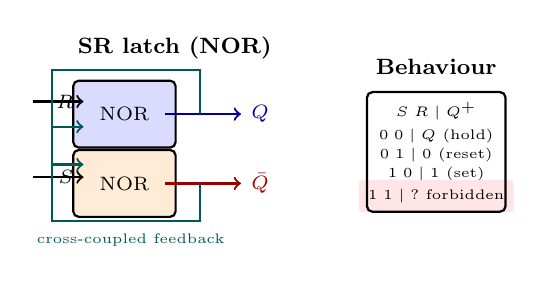
\begin{tikzpicture}[scale=0.80,every node/.style={font=\scriptsize}]
% SR latch NOR
\node[font=\footnotesize\bfseries] at (1.8,2.2) {SR latch (NOR)};
\node[draw,thick,fill=blue!14,minimum width=1.3cm,minimum height=0.85cm,rounded corners=2pt] (nor1) at (1.0,1.15) {NOR};
\node[draw,thick,fill=orange!16,minimum width=1.3cm,minimum height=0.85cm,rounded corners=2pt] (nor2) at (1.0,0.05) {NOR};
\draw[->,thick] (-0.45,1.35)--(0.35,1.35) node[left] {$R$};
\draw[->,thick] (-0.45,0.15)--(0.35,0.15) node[left] {$S$};
\draw[->,thick,blue!60!black] (1.65,1.15)--(2.85,1.15) node[right] {$Q$};
\draw[->,thick,red!60!black] (1.65,0.05)--(2.85,0.05) node[right] {$\bar Q$};
% feedback
\draw[->,thick,teal!70!black] (2.2,1.15)--(2.2,1.85)--(-0.15,1.85)--(-0.15,0.35)--(0.35,0.35);
\draw[->,thick,teal!70!black] (2.2,0.05)--(2.2,-0.55)--(-0.15,-0.55)--(-0.15,0.95)--(0.35,0.95);
\node[font=\tiny,teal!70!black] at (1.1,-0.85) {cross-coupled feedback};
% Truth table
\begin{scope}[xshift=4.8cm,yshift=0.15cm]
\node[font=\footnotesize\bfseries] at (1.15,1.75) {Behaviour};
\node[font=\tiny,align=left] at (1.15,1.05) {$S\;R\;|\;Q^+$};
\node[font=\tiny,align=left] at (1.15,0.65) {$0\;0\;|\;Q$ (hold)};
\node[font=\tiny,align=left] at (1.15,0.35) {$0\;1\;|\;0$ (reset)};
\node[font=\tiny,align=left] at (1.15,0.05) {$1\;0\;|\;1$ (set)};
\node[font=\tiny,align=left,fill=red!10,rounded corners=1pt] at (1.15,-0.30) {$1\;1\;|\;?$ forbidden};
\draw[thick,rounded corners=2pt] (0.05,1.35) rectangle (2.25,-0.55);
\end{scope}
\end{tikzpicture}
\caption{SR latch from cross-coupled NOR gates. Teal wires are feedback---the memory. Forbidden $S=R=1$ breaks bistability.}
\label{fig:sr-latch}
\end{figure}

Replacing NOR with NAND plus active-low inputs gives $\overline{S}\,\overline{R}$ latch,
the building block of many CMOS latches. Adding an enable $C$ gives the \emph{gated SR latch}:
when $C=0$ it holds; when $C=1$ it is transparent.

\section{D Latch: Removing the Forbidden State}
\label{sec:d-latch}
The \emph{D (data) latch} ties $R=\bar D$ so $S$ and $R$ never both $1$. One data input, one enable:
$C=1$ transparent ($Q=D$), $C=0$ hold. Solves SR's forbidden state at the cost of one lost
input combination.

\begin{figure}[h]
\centering
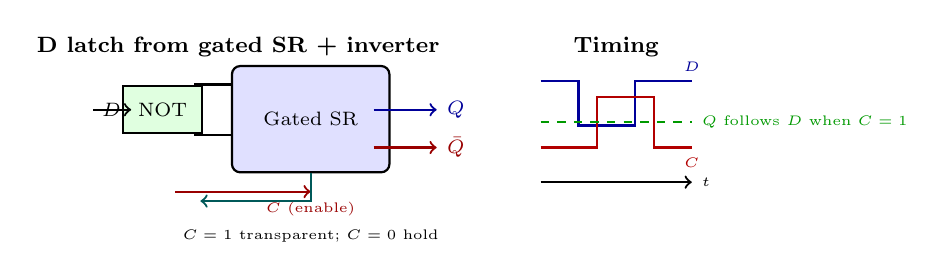
\begin{tikzpicture}[scale=0.80,every node/.style={font=\scriptsize}]
% D latch from SR
\node[font=\footnotesize\bfseries] at (2.0,2.15) {D latch from gated SR + inverter};
\node[draw,thick,fill=green!12,minimum width=1.0cm,minimum height=0.6cm] (inv) at (0.8,1.15) {NOT};
\draw[->,thick] (-0.3,1.15)--(0.3,1.15) node[left] {$D$};
\draw[->,thick] (1.3,1.55)--(2.1,1.55); \draw[->,thick] (1.3,0.75)--(2.1,0.75);
% SR block
\node[draw,thick,fill=blue!12,minimum width=2.0cm,minimum height=1.35cm,rounded corners=3pt] (sr) at (3.15,1.0) {Gated SR};
\draw[->,thick,red!60!black] (1.0,-0.15)--(3.15,-0.15) node[below,font=\tiny] {$C$ (enable)};
\draw[->,thick,teal!70!black] (3.15,0.15)--(3.15,-0.30)--(1.4,-0.30);
\draw[->,thick,blue!60!black] (4.15,1.15)--(5.15,1.15) node[right] {$Q$};
\draw[->,thick,red!60!black] (4.15,0.55)--(5.15,0.55) node[right] {$\bar Q$};
\node[font=\tiny,align=center] at (3.15,-0.85) {$C=1$ transparent; $C=0$ hold};
% Timing sketch
\begin{scope}[xshift=6.8cm]
\node[font=\footnotesize\bfseries] at (1.2,2.15) {Timing};
\draw[->,thick] (0,0)--(2.4,0) node[right,font=\tiny] {$t$};
\draw[thick,blue!60!black] (0,1.6)--(0.6,1.6)--(0.6,0.9)--(1.5,0.9)--(1.5,1.6)--(2.4,1.6) node[above,font=\tiny] {$D$};
\draw[thick,red!70!black] (0,0.55)--(0.9,0.55)--(0.9,1.35)--(1.8,1.35)--(1.8,0.55)--(2.4,0.55) node[below,font=\tiny] {$C$};
\draw[thick,green!60!black,dashed] (0,0.95)--(2.4,0.95) node[right,font=\tiny] {$Q$ follows $D$ when $C=1$};
\end{scope}
\end{tikzpicture}
\caption{D latch: one inverter eliminates the forbidden state. When $C=1$, $Q$ tracks $D$; when $C=0$, $Q$ holds.}
\label{fig:d-latch}
\end{figure}

\paragraph{Transparency problem.} A latch is \emph{level-sensitive}: while $C=1$, any glitch on $D$
propagates to $Q$. In multi-bit systems this causes races. The fix: make storage edge-triggered.

\section{From Latch to Flip-Flop}
\label{sec:flipflop}
\emph{Master-slave} pairs two D latches in series on opposite clock phases: master transparent
when $CLK=0$, slave when $CLK=1$---data ripples through only on the $0\!\to\!1$ edge.
Modern \emph{edge-triggered D flip-flop} ($\text{DFF}$) achieves the same with fewer transistors
(6 NAND gates) and is the standard library cell.

\begin{figure}[h]
\centering
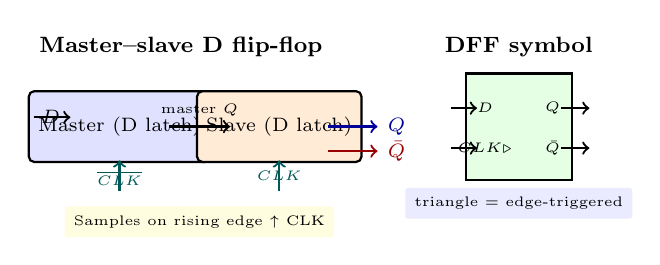
\begin{tikzpicture}[scale=0.78,every node/.style={font=\scriptsize}]
% Master-slave
\node[font=\footnotesize\bfseries] at (2.2,2.0) {Master--slave D flip-flop};
\node[draw,thick,fill=blue!12,minimum width=1.6cm,minimum height=0.9cm,rounded corners=2pt] (m) at (1.2,0.7) {Master (D latch)};
\node[draw,thick,fill=orange!16,minimum width=1.6cm,minimum height=0.9cm,rounded corners=2pt] (s) at (3.8,0.7) {Slave (D latch)};
\draw[->,thick] (-0.2,0.85)--(0.4,0.85) node[left] {$D$};
\draw[->,thick] (2.0,0.7)--(3.0,0.7) node[midway,above,font=\tiny] {master $Q$};
\draw[->,thick,blue!60!black] (4.6,0.7)--(5.4,0.7) node[right] {$Q$};
\draw[->,thick,red!60!black] (4.6,0.3)--(5.4,0.3) node[right] {$\bar Q$};
% Clock
\draw[->,thick,teal!70!black] (1.2,-0.35)--(1.2,0.15) node[below,font=\tiny] {$\overline{CLK}$};
\draw[->,thick,teal!70!black] (3.8,-0.35)--(3.8,0.15) node[below,font=\tiny] {$CLK$};
\node[font=\tiny,fill=yellow!12,rounded corners=1pt] at (2.5,-0.85) {Samples on rising edge $\uparrow$ CLK};
% DFF symbol
\begin{scope}[xshift=7.0cm]
\node[draw,thick,fill=green!10,minimum width=1.35cm,minimum height=1.35cm] (dff) at (0.7,0.7) {};
\node[font=\tiny] at (0.15,1.0) {$D$}; \node[font=\tiny] at (0.15,0.35) {$CLK\triangleright$};
\node[font=\tiny] at (1.25,1.0) {$Q$}; \node[font=\tiny] at (1.25,0.35) {$\bar Q$};
\draw[->,thick] (-0.4,1.0)--(0.02,1.0); \draw[->,thick] (-0.4,0.35)--(0.02,0.35);
\draw[->,thick] (1.38,1.0)--(1.85,1.0); \draw[->,thick] (1.38,0.35)--(1.85,0.35);
\node[font=\footnotesize\bfseries] at (0.7,2.0) {DFF symbol};
\node[font=\tiny,fill=blue!8,rounded corners=1pt] at (0.7,-0.55) {triangle = edge-triggered};
\end{scope}
\end{tikzpicture}
\caption{Master--slave construction and the standard D flip-flop symbol (triangle denotes edge-triggered clock).}
\label{fig:master-slave}
\end{figure}

\paragraph{JK and T flip-flops.} \emph{JK} generalises SR: $J$ sets, $K$ resets, $J=K=1$ toggles
($Q^+=\bar Q$). No forbidden state. \emph{T} (toggle) has one input: $T=1$ toggles, $T=0$ holds---ideal for counters (Ch.~\ref{ch:registers}).

\paragraph{Timing constraints.} \emph{Setup time} $t_{su}$: $D$ must be stable before the edge.
\emph{Hold time} $t_h$: $D$ must remain stable after the edge. \emph{Clock-to-Q} $t_{cq}$: delay from edge to new $Q$.
Violating $t_{su}/t_h$ risks \emph{metastability} (output hovers mid-rail).

\begin{definition}[Characteristic and excitation tables]
\emph{Characteristic:} $Q^+$ as function of inputs and $Q$. D: $Q^+=D$; JK: $Q^+=JQ'+\bar KQ$.
\emph{Excitation:} inputs required to get $Q\to Q^+$. D needs $D=Q^+$; JK needs $J,K$ pattern per transition.
\end{definition}


\section{Timing Analysis and Flip-Flop Variants in Practice}
Real flip-flops have \emph{propagation delay} $t_{cq}$ (clock to $Q$), \emph{setup} $t_{su}$ and \emph{hold} $t_h$.
For a register-to-register path with combinational delay $t_{comb}$,
\[ T_{clk} \ge t_{cq}+t_{comb}+t_{su},\qquad t_{hold}\le t_{cq}+t_{comb}^{\min}. \]
If $T_{clk}$ is too short, setup fails; if $t_{comb}^{\min}$ is too short, hold fails (often fixed by buffer insertion).
\emph{Asynchronous} preset/clear override the clock---useful for power-on reset but must be deasserted synchronously to avoid metastability.

\begin{example}[Choosing a flip-flop]
D is simplest for data-path registers (one data pin, no decode). JK/T shine where toggling is the natural operation
(counters, frequency dividers: $f_{out}=f_{clk}/2^n$ from $n$ cascaded T stages). In CMOS libraries, DFF is the default cell;
JK is built as D with feedback when needed.
\end{example}

% ============================================================

% ============================================================
\section{Chapter Notes}
The bistable latch dates to Eccles--Jordan (1918) vacuum-tube trigger circuit. Edge-triggered DFFs became
standard with TTL 7474 (1970s). Setup/hold analysis is essential for static timing analysis in modern ASIC flows.

% ============================================================
\section{Metastability and Synchronizers}
When setup/hold is violated (e.g.\ an asynchronous input sampled by a clock), a flip-flop can enter \emph{metastability}---output
hovers near $V_{DD}/2$ for unbounded time before resolving to $0$ or $1$. Probability decays exponentially with extra waiting time.
Fix: \emph{two-flop synchronizer} (cascade two DFFs on the receiving clock) gives one extra cycle for resolution; mean time between
failures (MTBF) grows by orders of magnitude. Never sample an async signal with a single flop in a reliable system.

% ============================================================

\section{Exercises}
\label{sec:ch04-exercises}
\begin{enumerate}[label=E4.\arabic*, leftmargin=*, itemsep=0.8em]
    \item \textbf{SR forbidden.} For the NOR SR latch, show the $S=R=1\to0$ transition can go metastable. Why does NAND SR have the same issue with $\bar S=\bar R=0$?
    \item \textbf{D latch timing.} Sketch $C$, $D$, $Q$ for $D$ toggling while $C=1$ then holding while $C=0$. Mark where transparency lets a glitch through.
    \item \textbf{JK analysis.} Derive $Q^+=JQ'+\bar KQ$ from the JK truth table. Show $T$ is JK with $J=K=T$, and D is JK with $J=D$, $K=\bar D$.
    \item \textbf{Setup/hold.} A DFF has $t_{su}=20$\,ns, $t_h=10$\,ns, $t_{cq}=15$\,ns. Can a $50$\,MHz clock drive two DFFs in series without violation? What about $80$\,MHz?
    \item \textbf{Excitation.} Fill the excitation table for D, JK, and T flip-flops for all $Q\to Q^+$ transitions ($0\to0$, $0\to1$, $1\to0$, $1\to1$).
\end{enumerate}
% End of Chapter 4
